\section{Wstęp}
%\subsection{Geneza}
Tematem projektu, którego dotyczy ta praca jest: „Projekt i~realizacja stanowiska laboratoryjnego do badania zależności czasowych w~sieci EtherCAT". Zagadnienia związane z~tworzeniem oprogramowania dla sterowników przemysłowych są dla autora niezwykle interesujące, a zrealizowany projekt miał na~celu dalsze pogłębienie jego wiedzy z tego zakresu. Wyboru tego konkretnego tematu autor dokonał, ponieważ protokół EtherCAT jest jeszcze nowością i według wielu źródeł stanowi przyszłość branży informatyki przemysłowej \cite{art1, art2}, a~praca nad tym tematem wydaje się być pomocna i~wartościowa w przyszłej pracy zawodowej lub na~ewentualnym dalszym etapie kształcenia.

\subsection{Stanowisko laboratoryjne}
Na potrzeby realizacji projektu wykorzystano dwa różne istniejące stanowiska laboratoryjne, które składały się odpowiednio~z:
\begin{table}[!htb]
\begin{center}
\begin{tabular}{| p{0.5\textwidth} || p{0.5\textwidth} |}\hline
Stanowisko typu CP (Rysunek~\ref{stanowisko:cp}) & Stanowisko typu CX (Rysunek~\ref{stanowisko:cx})  \\\hline
\begin{enumerate}
\item 2~silniki AM3021-0C00-0000,
\item Wyspa EK1100 z~zestawem modułów~IO,
\item Napęd serwomechnizmów AX5203 (2~osiowy napęd),
\item Komputer przemysłowy C6925,
\item Zasilacz.
\end{enumerate}
&
\begin{enumerate}
\item 2~silniki AM3021-0C00-0000,
\item Wyspa EK1100 z~zestawem modułów IO,
\item Napęd serwomechnizmów AX5203 (2~osiowy napęd),
\item Modułowy komputer przemysłowy CX1020,
\item Zasilacz.
\end{enumerate}
\\\hline                                            
\end{tabular}
\end{center}
\vspace*{-6mm}
  \caption{Dostępne stanowiska laboratoryjne}
	\label{in}
\end{table}

\begin{figure}[htbp]
 \centering
        \tikzstyle{background grid}=[draw, black!50,step=.25cm]
	\begin{tikzpicture}[node distance=1cm, auto]%, show background grid]
	\tikzset{
    	mynode/.style={rectangle,rounded corners,draw=black, top color=white, bottom color=yellow!50,very thick, inner sep=1em, minimum size=3em, 		text centered, text width=3cm},
    	mynodemini/.style={rectangle,rounded corners,draw=black, top color=white, bottom color=yellow!50,very thick, inner sep=.5em, text centered},    	
	    myarrow/.style={->, >=latex', shorten >=1pt, thick},
	    myline/.style={-, =latex', shorten >=1pt, rounded corners, ultra thick},
	    mylabel/.style={text width=7em, text centered} 
	} 
	\node[mynode] (plc) {Komputer \\ przemysłowy C6925};  
	\node [left=of plc] (laptop) {
\includegraphics[width=3cm]{images/laptop}};
	\node[mynode, right=of plc] (zasilacz) {Zasilacz};
	\node[below=2cm of plc] (dummy) {}; 
	\node[mynode, left=of dummy] (io) {Wyspa EK1100 z~zestawem modułów IO};  	 	 	
 	\node[mynodemini, left=of io] (io2) {EL1004};
 	\node[mynodemini, above=2mm of io2] (io1) {EL4132};  	
 	\node[mynodemini, above=2mm of io1] (io0) {EK1100};
 	\node[mynodemini, below=2mm of io2] (io3) {EL2004}; 	 	
 	\node[mynodemini, below=2mm of io3] (io4) {EL2004};
 	\node[mynodemini, below=2mm of io4] (io5) {EL3102};
 	\node [fit=(io0) (io1) (io2) (io3) (io4) (io5)] (fit) {};  
 	%\draw [decorate, xshift=-20pt,line width=4pt] (fit.south east) -- (fit.north east);
	\draw [decorate,decoration={brace, mirror,amplitude=10pt}, line width=1pt] (fit.south east) -- (fit.north east);
	
	\node[mynode, right=of dummy] (naped) {Napęd \\ serwomechnizmów AX5203};
	\node[below=2cm of naped] (dummy2) {}; 
	\node[mynode, left=of dummy2, text width=4cm](silnik1){Silnik \\ AM3021-0C00-0000};
	\node[mynode, right=of dummy2, text width=4cm](silnik2){Silnik \\ AM3021-0C00-0000};
	
	\draw[myline,black,dotted] (fit.east) ++(0.4, 0) -- (io.west);
	\draw[myline,blue] (laptop.east) -- ++(-1, 0) -- (plc.west);
	
	\draw[myline,black] (zasilacz.west) -- (plc.east);
	\draw[myline,black] (zasilacz.south) -- (io.north);
	\draw[myline,black] (zasilacz.south) -- (naped.north);	
	
	\draw[myline,purple] (io0.south) -- (io1.north);	
	\draw[myline,purple] (io1.south) -- (io2.north);
	\draw[myline,purple] (io2.south) -- (io3.north);		
	\draw[myline,purple] (io3.south) -- (io4.north);
	\draw[myline,purple] (io4.south) -- (io5.north);
	
	\draw[myline,yellow] (plc.south) -- (naped.north);	
	\draw[myline,yellow] (io.east) -- (naped.west);	

	\draw[myline, green, bend right=10] (naped.south) to (silnik1.north);
	\draw[myline, orange, bend left=10] (naped.south) to (silnik1.north);	
	\draw[myline, green, bend right=10] (naped.south) to (silnik2.north);
	\draw[myline, orange, bend left=10] (naped.south) to (silnik2.north);	
	%\draw[<->, >=latex', shorten >=2pt, shorten <=2pt, bend right=45, thick, dashed] 
    %(io.south) to node[auto, swap] {Competition}(naped.south); 
    
    \draw [purple, line width=6] (6,-1) -- (6.5,-1); \node[text width=2cm] at (7.65,-1.3) {EtherCAT (E-bus)};    
    \draw [yellow, line width=6] (6,-2) -- (6.5,-2); \node[text width=2cm] at (7.65,-2.3) {EtherCAT (skrętka)};
    \draw [blue, line width=6] (6,-3) -- (6.5,-3); \node at (7.5,-3) {Ethernet};
    \draw [black, line width=6] (6,-3.5) -- (6.5,-3.5); \node at (7.5,-3.5) {Zasilanie};
    \draw [green, line width=6] (6,-4) -- (6.25,-4); \draw [orange, line width=6] (6.25,-4) -- (6.5,-4); 
    \node [text width=2cm] at (7.75,-4.25) {Sterowanie silnikiem};    
\end{tikzpicture} 
\caption{Schemat stanowiska typu CP}
\label{stanowisko:cp}
\end{figure} %
\begin{figure}[htbp]
 \centering
        \tikzstyle{background grid}=[draw, black!50,step=.5cm]
	\begin{tikzpicture}[node distance=1cm, auto]%, show background grid]
	\tikzset{
    	mynode/.style={rectangle,rounded corners,draw=black, top color=white, bottom color=yellow!50,very thick, inner sep=1em, minimum size=3em, 		text centered, text width=3cm},
    	mynodemini/.style={rectangle,rounded corners,draw=black, top color=white, bottom color=yellow!50,very thick, inner sep=.5em, text centered},
	    myarrow/.style={->, >=latex', shorten >=1pt, thick},
	    myline/.style={-, =latex', shorten >=1pt, rounded corners, ultra thick},
	    mylabel/.style={text width=7em, text centered} 
	} 
	\node[mynode] (plc) {Modułowy komputer przemysłowy CX1020};  
	\node[mynode, above=of plc] (plc1) {CX1020-N010 \\ DVI/USB};
	\node[mynode, left=of plc1] (plc2) {CX1020-N000 \\ LAN};
	\node[mynode, right=of plc1] (plc3) {CX1020-0113 \\ CPU};
 	\node [fit=(plc1) (plc2) (plc3)] (fit) {}; 
 	\draw [decorate,decoration={brace,amplitude=10pt}, line width=1pt] (fit.south east) -- (fit.south west);
 		
	\node [left=of plc] (laptop) {
\includegraphics[width=3cm]{images/laptop}};
	\node[below=2cm of plc] (dummy) {}; 
	\node[mynode, left=of dummy] (io) {Zestaw  \\modułów~IO}; 
 	\node[mynodemini, left=of io] (io2) {EL1004};
	\node[mynodemini, above=2mm of io2] (io1) {EL4132};  	
 	\node[mynodemini, above=2mm of io1] (io0) {CX1100}; 	 	
 	\node[mynodemini, below=2mm of io2] (io3) {EL2004}; 	 	
 	\node[mynodemini, below=2mm of io3] (io4) {EL2004};
 	\node[mynodemini, below=2mm of io4] (io5) {EL3102};
 	\node [fit=(io0) (io1) (io2) (io3) (io4) (io5)] (fit2) {};  
 	%\draw [decorate, xshift=-20pt,line width=4pt] (fit.south east) -- (fit.north east);
	\draw [decorate,decoration={brace, mirror,amplitude=10pt}, line width=1pt] (fit2.south east) -- (fit2.north east);
 	 	 	 	 	 	
	\node[mynode, below=5mm of io, text width=1.6cm] (ek) {Terminal EK1100};  
	
	\node[mynode, right=of dummy] (naped) {Napęd \\ serwomechnizmów AX5203};
	\node[below=2cm of naped] (dummy2) {}; 
	\node[mynodemini, left=2mm of dummy2, text width=4cm](silnik1){Silnik \\ AM3021-0C00-0000};
	\node[mynodemini, right=2mm of dummy2, text width=4cm](silnik2){Silnik \\ AM3021-0C00-0000};

	\draw[myline,black,dotted] (fit.south) ++(0, -0.4) -- (plc.north);	
	\draw[myline,black,dotted] (fit2.east) ++(0.4, 0) -- (io.west);
	\draw[myline,blue] (laptop.east) -- ++(-1, 0) -- (plc.west);
	
	\draw[myline,purple] (plc.south) -- (io.north);	
	\draw[myline,purple] (io.south) -- (ek.north);
	\draw[myline,purple] (io0.south) -- (io1.north);	
	\draw[myline,purple] (io1.south) -- (io2.north);
	\draw[myline,purple] (io2.south) -- (io3.north);		
	\draw[myline,purple] (io3.south) -- (io4.north);
	\draw[myline,purple] (io4.south) -- (io5.north);
				
	\draw[myline,yellow] (ek.east) -- (naped.west);	

	\draw[myline, green, bend right=10] (naped.south) to (silnik1.north);
	\draw[myline, orange, bend left=10] (naped.south) to (silnik1.north);	
	\draw[myline, green, bend right=10] (naped.south) to (silnik2.north);
	\draw[myline, orange, bend left=10] (naped.south) to (silnik2.north);	
	%\draw[<->, >=latex', shorten >=2pt, shorten <=2pt, bend right=45, thick, dashed] 
    %(io.south) to node[auto, swap] {Competition}(naped.south); 
    
    \draw [purple, line width=6] (6,-1) -- (6.5,-1); \node[text width=2cm] at (7.65,-1.3) {EtherCAT (E-bus)};    
    \draw [yellow, line width=6] (6,-2) -- (6.5,-2); \node[text width=2cm] at (7.65,-2.3) {EtherCAT (skrętka)};
    \draw [blue, line width=6] (6,-3) -- (6.5,-3); \node at (7.5,-3) {Ethernet};
    \draw [black, line width=6] (6,-3.5) -- (6.5,-3.5); \node at (7.5,-3.5) {Zasilanie};
    \draw [green, line width=6] (6,-4) -- (6.25,-4); \draw [orange, line width=6] (6.25,-4) -- (6.5,-4); 
    \node [text width=2cm] at (7.75,-4.25) {Sterowanie silnikiem};    
\end{tikzpicture} 
\caption{Schemat stanowiska typu CX.}
\label{stanowisko:cx}
\end{figure}
 %

\subsubsection{Sterownik PLC}
Sterownik PLC wykorzystywany do realizacji projektu był wyposażony w następujące moduły:
\begin{enumerate}
\item SIMATIC S7-300, Jednostka centralna S7-300 CPU 315F-2 PN/DP,
\item SIMATIC S7-300, Zasilacz PS 307,
\item SIMATIC S7-300, Wejścia/Wyjścia cyfrowe SM 323,
\item SIMATIC S7-300, Wejścia/Wyjścia analogowe SM 334.
\end{enumerate}
%\begin{figure}[!htb] 	\centering 	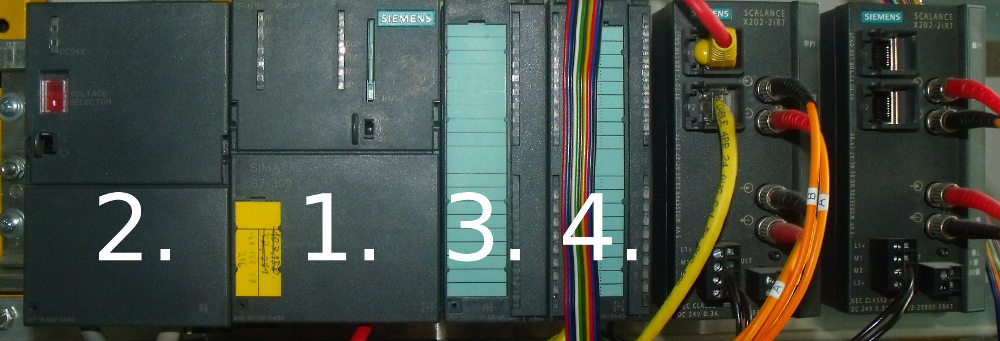
\includegraphics[width=0.75\textwidth]{obrazki/sterownik.png} 	\caption{Siemens SIMATIC S7-300} \end{figure}
\indent
\indent Sterownik podłączony jest do sieci lokalnej Ethernet w~laboratorium, więc komunikacja z~nim odbywa się tak samo jak z~każdym innym urządzeniem sieciowym. Podstawy programowania i korzystania ze sterowników autor poznał zapoznając się z odpowiednią literaturą \cite{plc1,plc2,plc4,plc5,plc6}.
Konfigurację sterownika wraz z modułami przedstawia Rysunek~\ref{conf}.
%\begin{figure}[!htb] 	\centering 	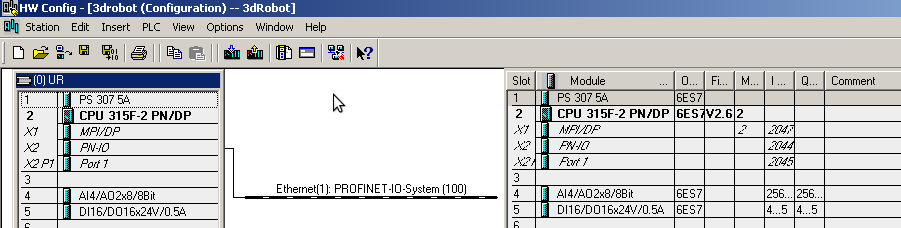
\includegraphics[width=0.75\textwidth]{obrazki/conf.png} \caption{Konfiguracja sterownika PLC} \label{conf} \end{figure}
\subsubsection{Komputer}
Projekt w całości był realizowany na laptopie autora, podłączanym do~sieci w~laboratorium. Na~komputerze uruchomiane były dwie maszyny wirtualne. Na~jednej zainstalowane było środowisko Step~7 do~programowania sterownika, a~na~drugiej WinCC flexible 2008 do~tworzenia i~uruchamiania wizualizacji. Wizualizacje tworzone w środowisku WinCC flexible są~dedykowane do~paneli operatorskich, jednak ta~stworzona przez autora na~potrzeby projektu była uruchamiana na komputerze za~pomocą runtime system.

!!!!!!!!
%\subsection{•}
\subsection{Analiza tematu}
Analiza tematu polegała przede wszystkim na zapoznaniu się z~narzędziami programistycznymi do~tworzenia oprogramowania sterownika oraz wizualizacji.
W~wyniku analizy autor poznał podstawy języków: LAD~\cite{step1,step2,step3}, STL~\cite{step1,step2,step3}, FBD~\cite{step1,step2,step3}, GRAPH~\cite{step3}, SCL~\cite{scl1,scl2,scl3} i AWL do~tworzenia programu sterownika oraz VBScript do~tworzenia skryptów w~wizualizacji.
Poznanie tych podstaw pozwoliło dobrać język odpowiedni do~realizacji poszczególnych zadań.

\subsection{Założenia}
Oprogramowanie dla dostępnego stanowiska laboratoryjnego powinno zostać stworzone przy użyciu środowiska TwinCAT. Funkcjonalności robota wchodzące w~skład projektu, to:
\begin{itemize}
\item sterowanie ręczne z~pilota podłączonego bezpośrednio do~sterownika,
\item sterowanie ręczne z~wizualizacji,
\item sterowanie automatyczne, 
\item wizualizacja stanu stanowiska.
\end{itemize}
\indent
\indent Powyżej zostały wymienione założenia podstawowe, jednak autor nie wyklucza zrealizowania dodatkowych zadań, które nie zostały zamieszczone w~pierwotnej koncepcji realizacji projektu.

\subsection{Plan pracy}
Realizacja projektu została podzielona na następujące etapy:
\begin{itemize}
\item Zapoznanie się ze sterownikami Beckhoff oraz oprogramowaniem TwinCAT,
\item Zapoznanie się z dostępnymi serwonapędami Beckhoff,
\item Projekt i realizacja stanowiska,
\item Przygotowanie stanowiska do współpracy z systemem wizualizacji,
\item Testowanie i uruchamianie,
\item Przedstawienie projektu i~ewentualne korekty.
\end{itemize}
\indent
\indent Powyższy plan pracy stanowił dla autora wyznacznik kolejnych działań. Jednak powszechnie wiadomo, że w~praktyce poszczególne punkty są~wymienne i~wpływają na siebie wzajemnie.
